\subsection{Mécaniques de jeu}

        \subsubsection{Environement}
            Nous nous sommes beaucoup inspirés du mode multijoueur des premiers Assassin's Creed.
            Le système de grimpe s'étant montré trop complexe à mettre en place, 
            nous avons réutilisé quelques idées de gameplay pour l'environement, comme les échelles et les portes.\\

            \begin{figure}[hbt!]
                \centering
                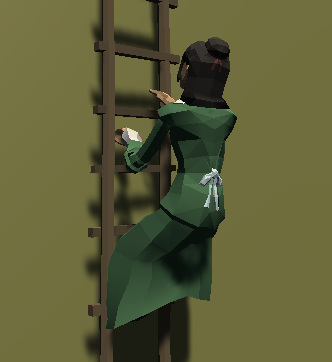
\includegraphics{ladder.png}
                \caption{Joueur grimpant sur l'échelle}
            \end{figure}

            Les échelles permettent de créer un peu de verticalité dans nos niveaux.
            Elles ne peuvent être utilisées que par les joueurs, mais ont leurs avantages comme leurs inconvénients : ainsi,
            prendre de la hauteur permet d'emprunter des raccourcis, mais retire la discrétion (car personne de civilisé devrait être sur les toits !) \\
            
            Les portes permettent de barrer le passage pour échapper à son agresseur.
            Elles se ferment quand le joueur passe dessus en courant
            et se rouvrent au bout de quelques secondes.

            \begin{figure}[ht]
                \centering
                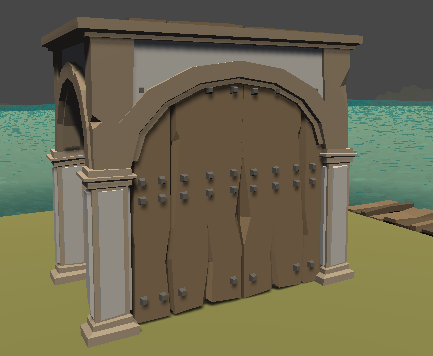
\includegraphics{doors_closed.png}
                \caption{Porte fermée après le passage d'un joueur}
            \end{figure}

            Ces interractions environnementales ont été réalisé par Renaud-Dov.

        \subsubsection{Déplacement du personnage}
            C'est Renaud-Dov qui a réalisé les contrôles de déplacement du personnage:
        
            Tout jeu est très rapidement limité par la capacité de déplacement du personnage et sa vitesse.
            Nous avons donc réalisé un script de déplacement qui permet au joueur de marcher, courir, sauter et grimper aux échelles.\\

            Pour le côté technique, nous avons dans un premier temps utilisé l'Input System de base proposé par Unity. Mais plusieurs problèmes se sont posés:
            \begin{itemize}
                \item Les configurations des keymaps sont assez limitées
                \item Paramétrer des périphériques autre que le clavier/souris est compliqué. Il faudrait avoir des scripts différents pour chaque périphérique, et donc des prefabs différents
            \end{itemize}
            C'est pour cette raison que nous avons migré vers le New Input System.
            Celui ci est ergonomique, multiplateformes et permet l'utilisation de différents périphériques, comme la manette ou le clavier par exemple.
            Certains scripts ont dû être modifiés pour devenir compatibles avec ce système.

            Il est donc actuellement possible de jouer au clavier/souris ou à la manette (pas les deux à fois).
            
        \subsubsection{Attribution des cibles}
            
            Harrys a réalisé le script permettant l'attribution des cibles, qui utilise des méthodes RPC (communication inter-clients par l'intermédiaire d'un serveur). Le "MasterClient", un client qui est désigné dans chaque salle pour faire office de maître de jeu, est celui qui séléctionne la cible de chaque joueur. Il communique ensuite à chacun des clients présents dans la salle sa cible désignée. Cette attribution se fait de façon aléatoire, mais selon certaines règles:
                
                -Un joueur ne peut (évidemment) pas être sa propre cible
                -Deux joueurs ne peuvent pas être la cible l'un de l'autre (Cela permet une plus grande interaction entre les joueurs et pas simplement des scénarios en "1 contre 1").
                -Plusieurs joueurs ne peuvent pas avoir la même cible.
                
            Cependant même si ce script est fonctionnel, il n'a pas encore été implémenté. 
            Le système d'élimination de la cible fera l'objet d'un travail important pour la prochaine soutenance.
        
        
        \subsubsection{Système de verrouilage}
            
            Le système qui attribue des cibles à chaque joueur n'est pas entièrement implémenté, mais le joueur peut déjà tuer une cible, qu'elle soit la bonne ou non.
            Pour cela, il passe en mode verrouilage, et les personnages pointés par le viseur surbrillent.
            Pour les sélectionner, un coup de molette suffit, et le contour devient alors jaune, pour indiquer que la cible est verouillée.
            Il suffit alors d'être à moins d'un mètre pour l'éliminer.

            \begin{figure}[hbt!]
                \centering
                \begin{subfigure}[b]{0.3\textwidth}
                    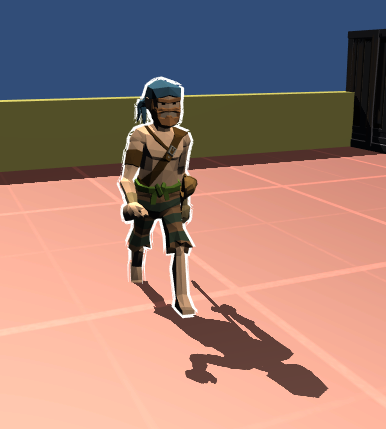
\includegraphics[scale=0.5]{white_outline.png} 
                    \caption{Personnage au centre de l'écran en surbrillance}
                \end{subfigure}
                \hspace{150pt}
                \begin{subfigure}[b]{0.3\textwidth}
                    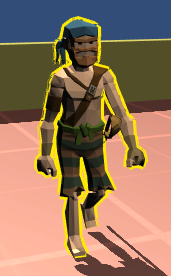
\includegraphics[scale=0.8]{yellow_outline.png} 
                    \caption{Personnage sélectionné et verrouilé}
                \end{subfigure}

                \begin{subfigure}[b]{0.3\textwidth}
                    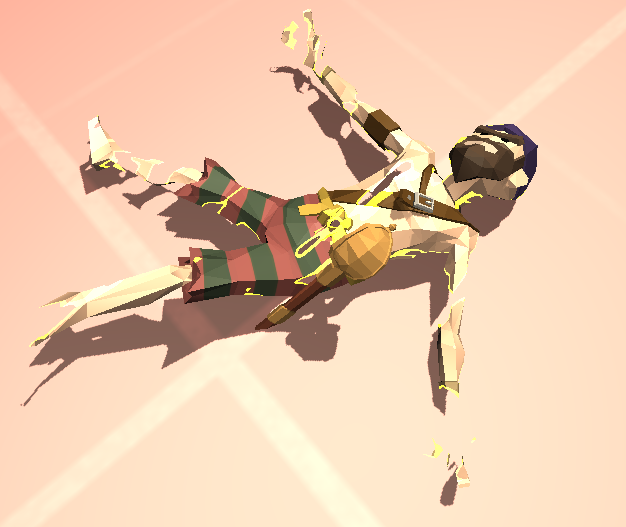
\includegraphics[scale=0.4]{death.png} 
                    \caption{Disparition des corps après mort}
                \end{subfigure}
                \caption{Système de verrouilage}
            \end{figure}

            Pour le matériau qui fait disparaitre les corps, nous avons créé manuellement un shader avec l'outil Shader Graph de Unity.

            Nous pouvons donc créer des shaders personalisés et dynamique (exemple utilisation du temps)

            \begin{figure}[hbt!]
                \centering
                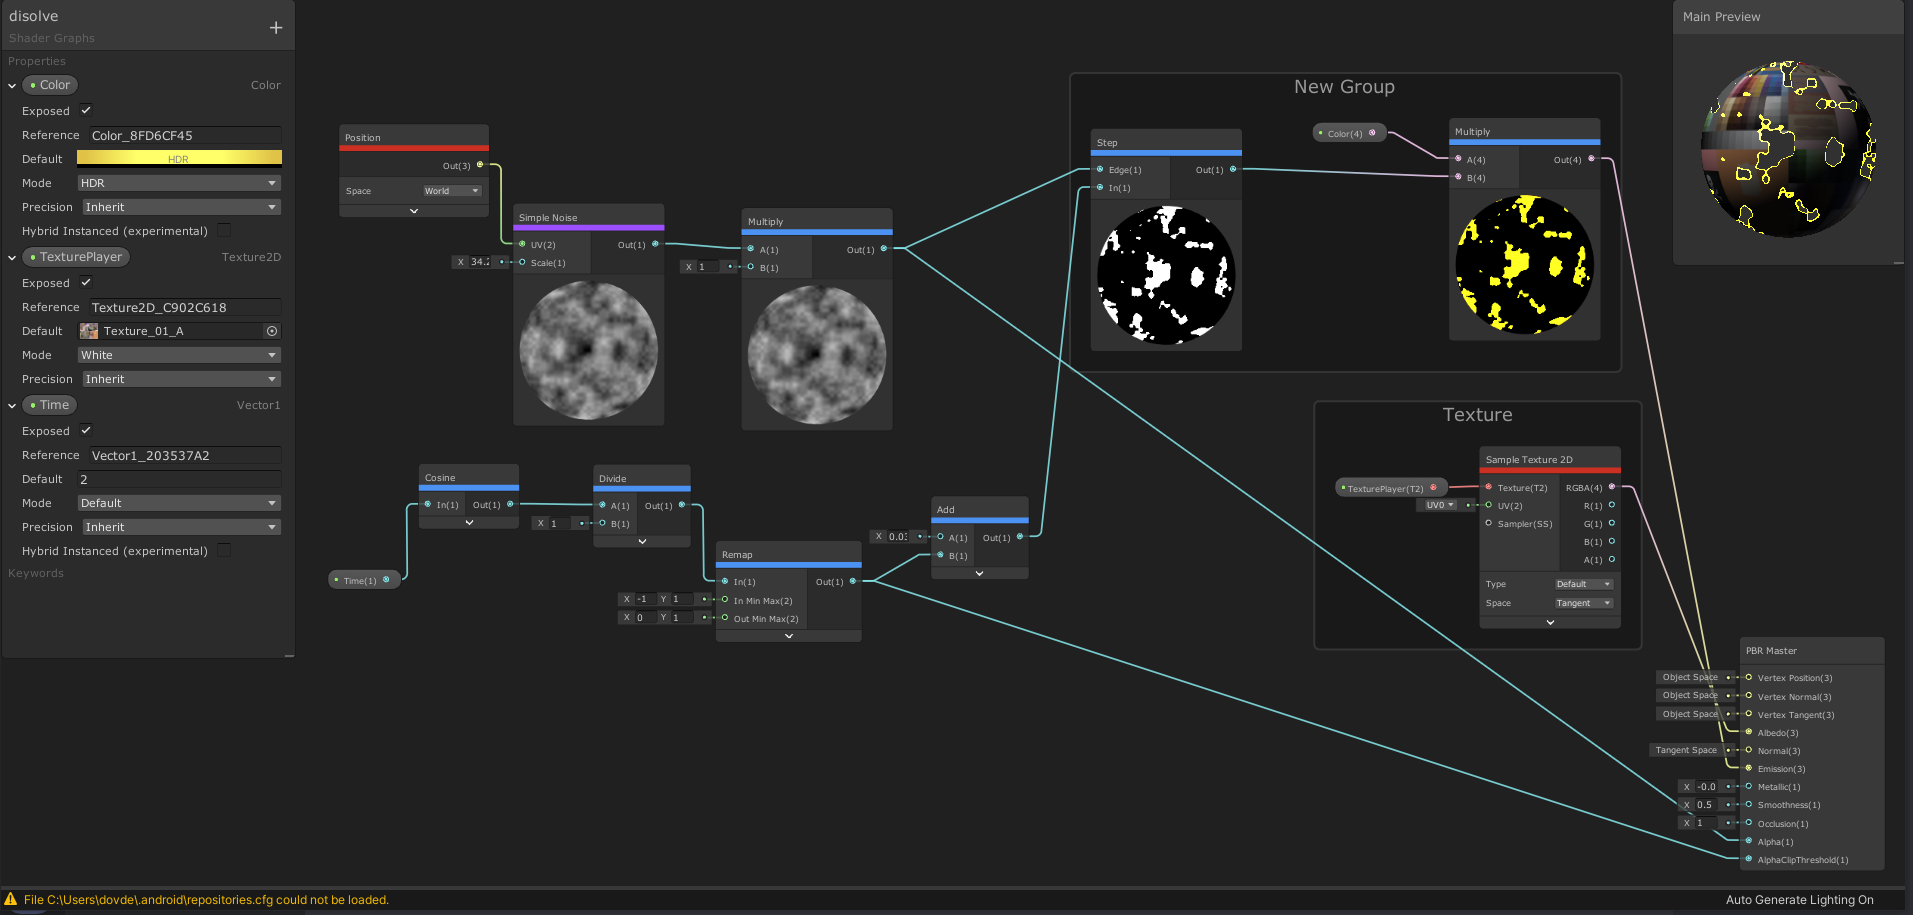
\includegraphics[scale=0.3]{dissolve_shader.png} 
            \end{figure}